\chapter{راهنمای استفاده از الگوی لاتک دانشگاه صنعتی امیرکبیر(پلی‌تکنیک تهران)}

\section{مقدمه}
حروف‌چینی پروژه کارشناسی، پایان‌نامه یا رساله یکی از موارد پرکاربرد استفاده از زی‌پرشین است. از طرفی، یک پروژه، پایان‌نامه یا رساله،  احتیاج به تنظیمات زیادی از نظر صفحه‌آرایی  دارد که ممکن است برای
یک کاربر مبتدی، مشکل باشد. به همین خاطر، برای راحتی کار کاربر، یک کلاس با نام 
\verb;AUTthesis;
 برای حروف‌چینی پروژه‌ها، پایان‌نامه‌ها و رساله‌های دانشگاه صنعتی امیرکبیر با استفاده از نرم‌افزار زی‌پرشین،  آماده شده است. این فایل به 
گونه‌ای طراحی شده است که کلیه خواسته‌های مورد نیاز  مدیریت تحصیلات تکمیلی دانشگاه صنعتی امیرکبیر را برآورده می‌کند و نیز، حروف‌چینی بسیاری
از قسمت‌های آن، به طور خودکار انجام می‌شود.

کلیه فایل‌های لازم برای حروف‌چینی با کلاس گفته شده، داخل پوشه‌ای به نام
\verb;AUTthesis;
  قرار داده شده است. توجه داشته باشید که برای استفاده از این کلاس باید فونت‌های
  \verb;Nazanin B;،
 \verb;PGaramond;
 و
  \verb;IranNastaliq;
    روی سیستم شما نصب شده باشد.
\section{این همه فایل؟!}\label{sec2}
از آنجایی که یک پایان‌نامه یا رساله، یک نوشته بلند محسوب می‌شود، لذا اگر همه تنظیمات و مطالب پایان‌نامه را داخل یک فایل قرار بدهیم، باعث شلوغی
و سردرگمی می‌شود. به همین خاطر، قسمت‌های مختلف پایان‌نامه یا رساله  داخل فایل‌های جداگانه قرار گرفته است. مثلاً تنظیمات پایه‌ای کلاس، داخل فایل
\verb;AUTthesis.cls;، 
تنظیمات قابل تغییر توسط کاربر، داخل 
\verb;commands.tex;،
قسمت مشخصات فارسی پایان‌نامه، داخل 
\verb;fa_title.tex;,
مطالب فصل اول، داخل 
\verb;chapter1;
و ... قرار داده شده است. نکته مهمی که در اینجا وجود دارد این است که از بین این  فایل‌ها، فقط فایل 
\verb;AUTthesis.tex;
قابل اجرا است. یعنی بعد از تغییر فایل‌های دیگر، برای دیدن نتیجه تغییرات، باید این فایل را اجرا کرد. بقیه فایل‌ها به این فایل، کمک می‌کنند تا بتوانیم خروجی کار را ببینیم. اگر به فایل 
\verb;AUTthesis.tex;
دقت کنید، متوجه می‌شوید که قسمت‌های مختلف پایان‌نامه، توسط دستورهایی مانند 
\verb;input;
و
\verb;include;
به فایل اصلی، یعنی 
\verb;AUTthesis.tex;
معرفی شده‌اند. بنابراین، فایلی که همیشه با آن سروکار داریم، فایل 
\verb;AUTthesis.tex;
است.
در این فایل، فرض شده است که پایان‌نامه یا رساله شما، از5 فصل و یک پیوست، تشکیل شده است. با این حال، اگر
  پایان‌نامه یا رساله شما، بیشتر از 5 فصل و یک پیوست است، باید خودتان فصل‌های بیشتر را به این فایل، اضافه کنید. این کار، بسیار ساده است. فرض کنید بخواهید یک فصل دیگر هم به پایان‌نامه، اضافه کنید. برای این کار، کافی است یک فایل با نام 
\verb;chapter6;
و با پسوند 
\verb;.tex;
بسازید و آن را داخل پوشه 
\verb;AUTthesis;
قرار دهید و سپس این فایل را با دستور 
\texttt{\textbackslash include\{chapter6\}}
داخل فایل
\verb;AUTthesis.tex;
و بعد از دستور
\texttt{\textbackslash include\{chapter6\}}
 قرار دهید.

\section{از کجا شروع کنم؟}
قبل از هر چیز، بدیهی است که باید یک توزیع تِک مناسب مانند 
\verb;Live TeX;
و یک ویرایش‌گر تِک مانند
\verb;Texmaker;
را روی سیستم خود نصب کنید.  نسخه بهینه شده 
\verb;Texmaker;
را می‌توانید  از سایت 
 \href{http://www.parsilatex.com}{پارسی‌لاتک}%
\LTRfootnote{\url{http://www.parsilatex.com}}
 و
\verb;Live TeX;
را هم می‌توانید از 
 \href{http://www.tug.org/texlive}{سایت رسمی آن}%
\LTRfootnote{\url{http://www.tug.org/texlive}}
 دانلود کنید.
 
در مرحله بعد، سعی کنید که  یک پشتیبان از پوشه 
\verb;AUTthesis;
 بگیرید و آن را در یک جایی از هارددیسک سیستم خود ذخیره کنید تا در صورت خراب کردن فایل‌هایی که در حال حاضر، با آن‌ها کار می‌کنید، همه چیز را از 
 دست ندهید.
 
 حال اگر نوشتن پایان‌نامه اولین تجربه شما از کار با لاتک است، توصیه می‌شود که یک‌بار به طور سرسری، کتاب «%
\href{http://www.tug.ctan.org/tex-archive/info/lshort/persian/lshort.pdf}{مقدمه‌ای نه چندان کوتاه بر
\lr{\LaTeXe}}\LTRfootnote{\url{http://www.tug.ctan.org/tex-archive/info/lshort/persian/lshort.pdf}}»
   ترجمه دکتر مهدی امیدعلی، عضو هیات علمی دانشگاه شاهد را مطالعه کنید. این کتاب، کتاب بسیار کاملی است که خیلی از نیازهای شما در ارتباط با حروف‌چینی را برطرف می‌کند.
 
 
بعد از موارد گفته شده، فایل 
\verb;AUTthesis.tex;
و
\verb;fa_title;
را باز کنید و مشخصات پایان‌نامه خود مثل نام، نام خانوادگی، عنوان پایان‌نامه و ... را جایگزین مشخصات موجود در فایل
\verb;fa_title;
 کنید. دقت داشته باشید که نیازی نیست 
نگران چینش این مشخصات در فایل پی‌دی‌اف خروجی باشید. فایل 
\verb;AUTthesis.cls;
همه این کارها را به طور خودکار برای شما انجام می‌دهد. در ضمن، موقع تغییر دادن دستورهای داخل فایل
\verb;fa_title;
 کاملاً دقت کنید. این دستورها، خیلی حساس هستند و ممکن است با یک تغییر کوچک، موقع اجرا، خطا بگیرید. برای دیدن خروجی کار، فایل 
\verb;fa_title;
 را 
\verb;Save;، 
(نه 
\verb;As Save;)
کنید و بعد به فایل 
\verb;AUTthesis.tex;
برگشته و آن را اجرا کنید. حال اگر می‌خواهید مشخصات انگلیسی پایان‌نامه را هم عوض کنید، فایل 
\verb;en_title;
را باز کنید و مشخصات داخل آن را تغییر دهید.%
\RTLfootnote{
برای نوشتن پروژه کارشناسی، نیازی به وارد کردن مشخصات انگلیسی پروژه نیست. بنابراین، این مشخصات، به طور خودکار،
نادیده گرفته می‌شود.
}
 در اینجا هم برای دیدن خروجی، باید این فایل را 
\verb;Save;
کرده و بعد به فایل 
\verb;AUTthesis.tex;
برگشته و آن را اجرا کرد.

برای راحتی بیشتر، 
فایل 
\verb;AUTthesis.cls;
طوری طراحی شده است که کافی است فقط  یک‌بار مشخصات پایان‌نامه  را وارد کنید. هر جای دیگر که لازم به درج این مشخصات باشد، این مشخصات به طور خودکار درج می‌شود. با این حال، اگر مایل بودید، می‌توانید تنظیمات موجود را تغییر دهید. توجه داشته باشید که اگر کاربر مبتدی هستید و یا با ساختار فایل‌های  
\verb;cls;
 آشنایی ندارید، به هیچ وجه به این فایل، یعنی فایل 
\verb;AUTthesis.cls;
دست نزنید.

نکته دیگری که باید به آن توجه کنید این است که در فایل 
\verb;AUTthesis.cls;،
سه گزینه به نام‌های
\verb;bsc;,
\verb;msc;
و
\verb;phd;
برای تایپ پروژه، پایان‌نامه و رساله،
طراحی شده است. بنابراین اگر قصد تایپ پروژه کارشناسی، پایان‌نامه یا رساله را دارید، 
 در فایل 
\verb;AUTthesis.tex;
باید به ترتیب از گزینه‌های
\verb;bsc;،
\verb;msc;
و
\verb;phd;
استفاده کنید. با انتخاب هر کدام از این گزینه‌ها، تنظیمات مربوط به آنها به طور خودکار، اعمل می‌شود.

\section{مطالب پایان‌نامه را چطور بنویسم؟}
\subsection{نوشتن فصل‌ها}
همان‌طور که در بخش 
\ref{sec2}
گفته شد، برای جلوگیری از شلوغی و سردرگمی کاربر در هنگام حروف‌چینی، قسمت‌های مختلف پایان‌نامه از جمله فصل‌ها، در فایل‌های جداگانه‌ای قرار داده شده‌اند. 
بنابراین، اگر می‌خواهید مثلاً مطالب فصل ۱ را تایپ کنید، باید فایل‌های 
\verb;AUTthesis.tex;
و
\verb;chapter1;
را باز کنید و محتویات داخل فایل 
\verb;chapter1;
را پاک کرده و مطالب خود را تایپ کنید. توجه کنید که همان‌طور که قبلاً هم گفته شد، تنها فایل قابل اجرا، فایل 
\verb;AUTthesis.tex;
است. لذا برای دیدن حاصل (خروجی) فایل خود، باید فایل  
\verb;chapter1;
را 
\verb;Save;
کرده و سپس فایل 
\verb;AUTthesis.tex;
را اجرا کنید. یک نکته بدیهی که در اینجا وجود دارد، این است که لازم نیست که فصل‌های پایان‌نامه را به ترتیب تایپ کنید. می‌توانید ابتدا مطالب فصل ۳ را تایپ کنید و سپس مطالب فصل ۱ را تایپ کنید.

نکته بسیار مهمی که در اینجا باید گفته شود این است که سیستم
\lr{\TeX},
محتویات یک فایل تِک را به ترتیب پردازش می‌کند. به عنوان مثال، اگه فایلی، دارای ۴ خط دستور باشد، ابتدا خط ۱، بعد خط ۲، بعد خط ۳ و در آخر، خط ۴ پردازش می‌شود. بنابراین، اگر مثلاً مشغول تایپ مطالب فصل ۳ هستید، بهتر است
که دو دستور
\verb~\chapter{مقدمه}


بیشتر سرویس‌های شبکه بر روی سخت افزارهای اختصاصی به نام
\lr{middle box}
ساخته می‌شوند.
تنوع و تعداد رو به افزایش سرویس‌های جدیدی که توسط کاربران تقاضا می‌گردد
باعث هزینه‌های زیاد برای خرید و نگهداری
\lr{middle box}‌ها
توسط اپراتورها شده است.
به تازگی فراهم آورندگان شبکه
شروع به حرکت به سوی مجازی‌سازی و نرم‌افزاری کردن بسترهای شکبه کرده‌اند،
به این ترتیب آن‌ها قادر خواهند بود
سرویس‌های نوآورانه‌ای به کاربران ارائه بدهند.

مجازی‌سازی توابع شبکه‌ راهکاری است که برای همین منظور پیشنهاد شده است.
مجازی‌سازی توابع شبکه‌ در واقع راه‌حل‌های مشخصی را برای چالش‌های جای‌گذاری،
زنجیره‌سازی و هماهنگی سرویس‌های شبکه فراهم می‌آورد.

ایده‌ی اصلی مجازی‌سازی توابع شبکه جداسازی تجهیزات فیزیکی شبکه از کارکردهایی می‌باشد که
بر روی آن‌ها اجرا می‌شوند.
به این معنی که یک کاکرد شبکه مانند دیوار آتش می‌تواند بر روی یک
\lr{TSP}
به عنوان یک نرم‌افزار ساده فرستاده شود.
با این روش یک سرویس می‌تواند به مجموعه‌ای از کارکردهای مجازی شبکه‌ای که می‌توانند به صورت نرم‌افزاری پیاده‌سازی شده
و روی یک یا تعداد سرور استاندارد فیزیکی اجرا شوند، شکسته شود.
کارکرهای مجازی شبکه‌ای می‌توانند در مکان‌های مختلف بازمکان‌یابی یا نمونه‌سازی شوند بدون آنکه
نیاز به خریداری و نصب تجهیز جدیدی باشد.
\cite{Mijumbi2016}

\section{معماری \lr{NFV}}
با توجه به استاندارد \lr{ETSI} معماری \lr{NFV}
از سه عنصر کلیدی تشکیل شده است.~
و
\verb~\chapter{مفاهیم پایه}

\section{مقدمه}

راه اندازی و استقرار سرویس در صنعت مخابرات به طور سنتی بر این اساس است که اپراتورهای شبکه سخت‌افزارهای اختصاصی فیزیکی و تجهیزات لازم برای هر کارکرد در سرویس را در زیرساخت خود مستقر کنند.
فراهم کردن نیازمندی‌هایی مانند پایداری و کیفیت بالا منجر به اتکای فراهم کنندگان سرویس بر سخت‌افزارهای اختصاصی می‌شود. 
این درحالی است که نیازمندی کاربران به سرویس‌های متنوع و عموما با عمرکوتاه و نرخ بالای ترافیک افزایش یافته است.
بنابراین فراهم کنندگان سرویس‌ها باید مرتبا و به صورت پیوسته تجهیزات فیزیکی جدید را خریده، انبارداری کرده و مستقر کنند.
تمام این عملیات باعث افزایش هزینه های فراهم کنندگان سرویس می‌شود.
با افزایش تجهیزات، پیدا کردن فضای فیزیکی برای استقرار تجهیزات جدید به مرور دشوارتر می‌شود.
علاوه بر این باید افزایش هزینه و تاخیر ناشی از آموزش کارکنان برای کار با تجهیزات جدید را نیز در نظر گرفت.
بدتر این که هر چه نوآوری سرویس‌ها و فناوری شتاب بیشتری می‍گیرد، چرخه عمر سخت‌افزارها کوتاه‍تر می‍شود که مانع از ایجاد نوآوری در سرویس‌های شبکه می‌شود.

در روش سنتی استقرار سرویس شبکه، ترافیک کاربر باید از تعدادی کارکرد شبکه به ترتیب معینی عبور کند تا یک مسیر پردازش ترافیک ایجاد شود.
در حال حاضر این کارکردها به صورت سخت‌افزاری به یکدیگر متصل هستند و ترافیک با استفاده از جداول مسیریابی به سمت آن‌ها هدایت می‌شود.
چالش اصلی این روش در این است که استقرار و تغییر ترتیب کارکردها دشوار است.
به عنوان مثال، به مرور زمان با تغییر شرایط شبکه نیازمند تغییر همبندی و یا مکان کارکردها برای سرویس‌دهی بهتر به کاربران هستیم که نیاز به جا به جایی کارکردها و تغییر جداول مسیریابی دارد.
در روش سنتی این کار سخت و هزینه‌بر است که ممکن است خطاهای بسیاری در آن رخ دهد.
از جنبه دیگر، تغییر سریع سرویس‌های مورد نظر کاربران نیازمند تغییر سریع در ترتیب کارکردها است که در روش فعلی این تغییرات به سختی صورت گیرد.
بنابراین اپراتورهای شبکه نیاز به شبکه های قابل برنامه ریزی و ایجاد زنجیره سرویس کارکردها به صورت پویا پیدا کرده اند.

دو فناوری برای پاسخگویی به این چالش‌ها مطرح شد:

\begin{itemize}
    \item مجازی‌سازی کارکرد شبکه یا \lr{NFV}
    \item زنجیره‌سازی کارکردهای سرویس یا \lr{SFC}
\end{itemize}

با استفاده از مجازی‌سازی کارکردهای شبکه و اجرای آن‌ها بر روی سرورهای استاندارد با توان بالا،
امکان اجرای کارکردها بر روی سخت افزارهای عمومی را فراهم کرده است تا نیاز به تجهیزات سخت افزاری خاص منظوره کاهش یابد.
از طرف دیگر \lr{SFC} امکان تعریف زنجیره کارکردها را ارائه می‌کند که ایجاد
و انتخاب مسیرهای متفاوت برای پردازش ترافیک به صورت پویا و بدون ایجاد تغییر در زیرساخت فیزیکی را امکان‌پذیر می‌کند
با توجه به این فناوری‌ها، مسائل تحقیقاتی جدیدی مطرح شدند که از مهم‌ترین آن‌ها می‌توان تخصیص منابع بهینه به سرویس درخواستی کاربر را نام برد.

از آنجایی که از مفاهیم این فناور‌ی‌ها برای طراحی و تعریف مساله در این رساله استفاده شده است، نیازمند آشنایی با مفاهیم ابتدایی و اصول اولیه آن‌ها خواهیم بود.

بنابراین در این فصل به صورت خلاصه اجزای این فناوری‌ها را مرور خواهیم کرد و کاربردها، چالش‌ها و مسائل تحقیقاتی که در هر یک از این معماری‌ها وجود دارد را مورد بررسی قرار خواهیم داد.

\section{مجازی‌سازی کارکرد شبکه}

مجازی‌سازی کارکرد شبکه اصل جداسازی کارکرد شبکه به وسیله انتزاع سخت‌افزاری مجازی از سخت افزاری است که بر روی آن اجرا می‌شود.
هدف مجازی‌سازی کارکرد شبکه تغییر روش اپراتورهای شبکه در طراحی شبکه
با تکامل مجازی سازی استاندارد فناوری اطلاعات به منظور تجمیع تجهیزات شبکه
در سرورهای استاندارد، سوییچ‌ها و ذخیره‌سازها با توان بالا است.
یک سرور استاندارد با توان بالا سروری است که توسط اجزای استاندارد شده \lr{IT}،
مانند معماری \lr{x86}، ساخته شده و
در تعداد بالایی، مانند میلیون،
فروخته می‌شود.
ویژگی اصلی این سرورها این است که اجزای آن‌ها به راحتی از فروشندگان مختلف قابل خریداری و
تعویض است.
این تجهیزات می‌توانند در مراکز داده، گره‌های شبکه، یا مکان کاربران انتهایی قرار بگیرند.
این روند در
شکل
\ref{fig.6}
نیز توصیف شده است.

\begin{figure}[!h]
\center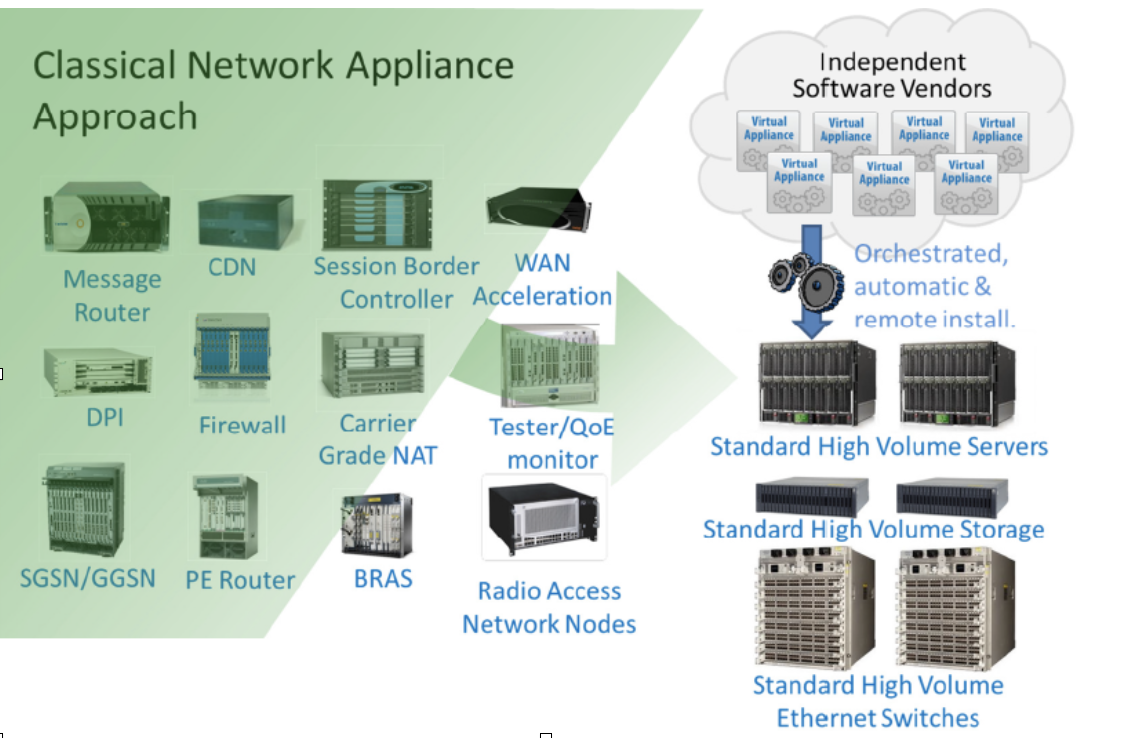
\includegraphics[scale=.5]{images/nfv-concept}
\caption{رویکرد \lr{NFV}}\label{fig.6}
\end{figure}

با استفاده از \lr{NFV}، انواع کارکردهای شبکه مانند دیواره آتش و \lr{NAT}
را می‌توان به صورت یک برنامه نرم‌افزاری از فروشندگان مختلف تهیه کرد و
آن‌ها را بر روی سرورهای با توان بالا اجرا کرد که نیاز به نصب تجهیزات خاص منظوره و
جدید را برطرف می‌سازد.

مزایا و اهداف اساسی که \lr{NFV} برای تحقق و دست‍یابی به آن‍ها شکل گرفته است عبارتند از:

\begin{itemize}
    \item
    کاهش هزینه‌های تجهیزات و مصرف انرژی از طریق تجمیع کارکردها بر روی سرورها و در نتیجه کاهش تعداد تجهیزات
    \item
    کاهش نیاز به آموزش کارکنان، افزایش دسترسی پذیری به سخت افزار و کاهش زمان بازیابی از خرابی سخت افزار به علت استفاده از سخت افزارهای استاندارد و عمومی
    \item
    افزایش سرعت عرضه محصول به بازار با کوتاه‌کردن چرخه نوآوری و تولید. در واقع \lr{NFV} به اپراتورهای شبکه کمک می‍کند تا چرخه بلوغ محصول را به اندازه قابل توجهی کاهش دهند.
    \item
    امکان‍پذیر بودن تعریف سرویس مورد نظر بر اساس نوع مشتری یا محل جغرافیایی. مقیاس سرویس‌ها می‍تواند به سرعت، بر اساس نیاز، گسترش یا کاهش یابد.
    \item
    تشویق به ایجاد نوآوری و ارائه سرویس‌های جدید و دریافت جریان‌های درآمدی تازه با سرعت بالا و ریسک پایین.
    \item
    افزایش توانایی  مقابله با خرابی کارکردها، قابلیت به اشتراک گذاری منابع بین کارکرد ها و پشتیابی از چند مشتری
\end{itemize}

سازمان‌های استانداردگذاری متعددی در استانداردسازی فناوری \lr{NFV} دخیل هستند که شاخص‌ترین آن‌ها موسسه استانداردهای مخابراتي اروپا (\lr{ETSI}) است.
در اواخر سال ۲۰۱۲،
\lr{ETSI NFV ISG}
توسط هفت اپراتور جهانی شبکه به منظور ارتقا ایده مجازی‌سازی کارکرد شبکه تأسیس شد.
\lr{NFV ISG}
تبدیل به یک بستر صنعتی اصلی برای توسعه چارچوب معماری \lr{NFV} و نیازمندی‌های آن شده است و اکنون بیش از ۲۵۰ سازمان با آن همکاری می‌کنند.
اسناد معماری \lr{NFV} به صورت عمومی و رایگان توسط \lr{ETSI NFV ISG} منتشر می‌شود.
ما در این رساله برای توصیف معماری \lr{NFV} از اسناد ارائه شده این سازمان استفاده می‌کنیم.

\section{معماری \lr{NFV}}

در این بخش مؤلفه‌های تشکیل‌دهنده معماری \lr{NFV} شرح داده می‍شوند.
هر یک از اجزای معماری می‍توانند توسط تولیدکنندگان متفاوتی تأمین شوند و به وسیله واسط‌هایی که توسط معماری \lr{NFV}
توصیف شده‌اند با یکدیگر در ارتباط باشند.
بنابراین معماری \lr{NFV} توصیف شده توسط \lr{ETSI} راه‌حلی با قابلیت مشارکت و هماهنگی چندین تولیدکننده مختلف را دارد.
با توجه به استاندارد \lr{ETSI} معماری \lr{NFV}
از سه عنصر کلیدی تشکیل شده است.
زیرساخت مجازی‌سازی کارکردهای شبکه،
کارکردهای مجازی شبکه‌ای و
\lr{NFV MANO}.
این اجزا در شکل \ref{fig.1} نمایش داده شده‌اند.

\begin{figure}[!h]
\center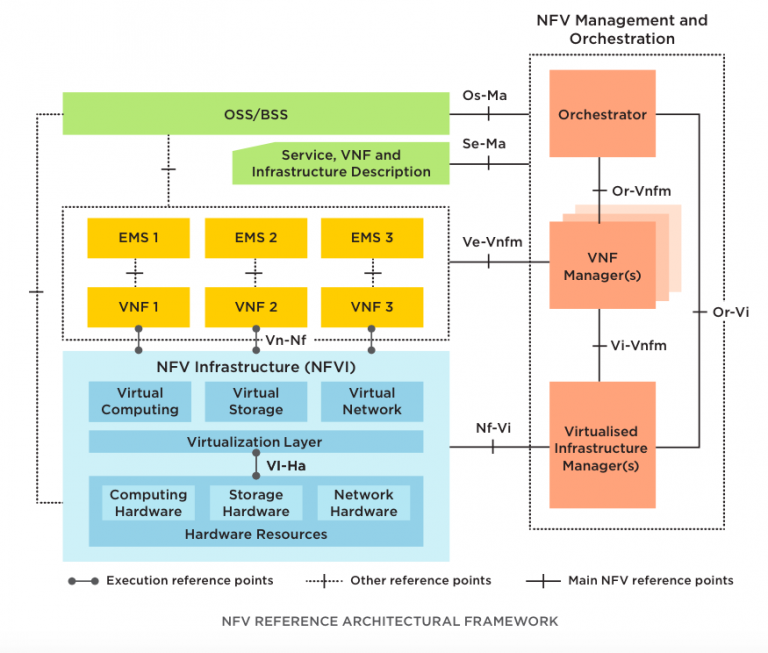
\includegraphics[scale=.5]{images/nfv-arch}
\caption{معماری مجازی‌سازی کارکردهای شبکه
}\label{fig.1}
\end{figure}

\begin{itemize}
    \item
    \lr{NFVI}: شامل منابع سخت افزاری و نرم‌افزاری لازم برای اجرای \lr{VNF}‌ها
    \item
    \lr{Service}: شامل \lr{VNF}‌ها که کارکردهای شبکه را پیاده‌سازی کرده‌اند، \lr{EMS} برای مدیریت \lr{VNF}‌ها و \lr{OSS/BSS} برای ارتباط با سیستم‌های مدیریت سنتی
    \item
    \lr{MANO}: که وظیفه مدیریت و هماهنگی سرویس‌ها و تخصیص منابع را برعهده دارد و از سه بخش \lr{NFVO}، \lr{VIM} و \lr{VNFM} تشکیل شده است.
\end{itemize}

\subsection{زیرساخت مجازی‌سازی کارکردهای شبکه یا \lr{NFVI}}
زیرساخت مجازی‌سازی کارکردهای شبکه ترکیبی از منابع نرم‌افزاری و سخت‌افزاری است
که محیطی برای نصب
کارکردهای مجازی شبکه فراهم می‌آورد.
منابع سخت‌افزاری شامل منابع محاسباتی،
ذخیره‌سازها و شبکه
(شامل لینک‌ها و گره‌ها)
هستند
که پردازش، ذخیره‌سازی و ارتباط را
برای کارکردهای مجازی شبکه فراهم می‌آورند.
منابع مجازی انتزاعی از منابع شبکه‌ای، پردازشی و ذخیر‌ه‌سازی هستند.
به وسیله انتزاع از طریق لایه‌ی مجازی‌سازی (بر پایه‌ی \lr{hypervisor})
منابع سخت افزاری در اختیار کارکردهای مجازی
قرار می‌گیرند که این منابع شامل منابع محاسباتی، شبکه‌ای و ذخیره‌سازی می‌باشند.

در مراکز داده‌ای ممکن است منابع پردازشی و ذخیره‌سازی تحت عنوان یک یا چند
ماشین مجازی نمایش داده شوند در حالی که شبکه‌های مجازی از لینک‌ها و گره‌های مجازی تشکیل می‌شوند.
شبکه‌های مجازی پیش از بحث مجازی‌سازی کارکردهای شبکه مدنظر بوده‌اند و روی آن‌ها کار شده است.
در واقع از شبکه‌های مجازی در مراکز داده‌ای جهت فراهم آوردن شبکه‌های مختلف و مجزا که به کاربران مختلفی تعلق دارند
استفاده شده است. راه‌حل‌های مختلفی برای پیاده‌سازی این شبکه‌ها وجود دارد. در بحث مجازی‌سازی کارکردهای شبکه‌، زیرساخت ارتباطی
مورد نیاز 
برای کارکردهای مجازی از طریق همین شبکه‌های مجازی فراهم آورده می‌شود.
یعنی مسائلی که پیشتر در بحث جایگذاری شبکه‌های مجازی مطرح بود
امروز جزئی از مسائل جایگذاری زنجیره‌های کارکرد سرویس می‌باشند.

\subsection{کارکردهای مجازی شبکه}
یک کارکرد شبکه، یک بلوک عملیاتی در زیرساخت شبکه است که عملکرد رفتاری و رابط‌های ارتباط با خارج خوش تعریف دارد.
مثال‌هایی از کارکردهای شبکه می‌تواند شامل
\lr{DHCP}
یا
\lr{firewall}
و ... باشد.
با این توضیحات کارکرد مجازی شبکه، پیاده‌سازی یک کارکرد شبکه است
که می‌تواند روی منابع مجازی شده اجرا شود.
از هر کارکرد شبکه می‌توان نمونه‌سازی کرده و چند نمونه را در شبکه مستقر ساخت. 
این نمونه‌ها می‌توانند برای سرویس‌دهی به زنجیره‌های مختلف استفاده شوند. از آنجایی که 
هر نمونه توان پردازشی محدودی دارد با افزایش تعداد نمونه‌ها می‌توان توان پردازشی یک کارکرد را نیز افزایش داد.

\subsection{\lr{EM}}
این مولفه کارکردهای \lr{FCAPS} را برای \lr{VNF} ها انجام می دهد که شامل مدیریت خطا، پیکربندی، امنیت، حسابداری و کارایی برای کارکردی است که \lr{VNF} ارائه می دهد. این مولفه ممکن است آگاه از مجازی کارکرد باشد و با همکاری \lr{VNFM} عملکردهای خودش را انجام بدهد.

\subsection{\lr{OSS/BSS}}
این مولفه، ترکیبی از سایر بخش های عملکردهای اپراتور است که در چارچوب معماری \lr{NFV} ارائه شده از طرف \lr{ETSI} قرار نمیگیرند. به عنوان مثال می تواند شامل مدیریت سیستم های \lr{Legacy} باشد.

\subsection{\lr{NFV MANO}}
بر اساس چهارچوب پیشنهادی \lr{ETSI}
وظیفه‌ی \lr{NFV MANO} فراهم آوردن کارکردهای لازم
برای تدارک و فرآیند‌های مشابه مانند تنظیم کردن و ... کارکردهای مجازی شبکه است.
\lr{NFV MANO} شامل هماهنگ کننده و مدیریت کننده چرخه‌ی زندگی
منابع سخت‌افزاری و نرم‌افزاری که مجازی‌سازی زیرساخت را پشتیبانی می‌کنند، است.
هر زنجیره نیاز دارد که حداقل توسط یک \lr{VNFM} مدیریت شود
تا مثلا خطاهای آن را تحت نظر قرار دهد و در صورت نیاز در قسمت دیگری از شبکه استقرار یابد.
مساله‌ی جایگذاری زنجیره‌ها بسیار مورد مطالعه قرار گرفته است، اما در این بین توجه لازم به نیاز این زنجیره‌ها به یک
\lr{VNFM}
صورت نپذیرفته است.
~
را در فایل 
\verb~AUTthesis.tex~،
غیرفعال%
\RTLfootnote{
برای غیرفعال کردن یک دستور، کافی است پشت آن، یک علامت
\%
 بگذارید.
}
 کنید. زیرا در غیر این صورت، ابتدا مطالب فصل ۱ و ۲ پردازش شده (که به درد ما نمی‌خورد؛ چون ما می‌خواهیم خروجی فصل ۳ را ببینیم) و سپس مطالب فصل ۳ پردازش می‌شود و این کار باعث طولانی شدن زمان اجرا می‌شود. زیرا هر چقدر حجم فایل اجرا شده، بیشتر باشد، زمان بیشتری هم برای اجرای آن، صرف می‌شود.

\subsection{مراجع}
برای وارد کردن مراجع به فصل 2
مراجعه کنید.
\subsection{واژه‌نامه فارسی به انگلیسی و برعکس}
برای وارد کردن واژه‌نامه فارسی به انگلیسی و برعکس، بهتر است مانند روش بکار رفته در فایل‌های 
\verb;dicfa2en;
و
\verb;dicen2fa;
عمل کنید.

\section{اگر سوالی داشتم، از کی بپرسم؟}
برای پرسیدن سوال‌های خود در مورد حروف‌چینی با زی‌پرشین،  می‌توانید به
 \href{http://forum.parsilatex.com}{تالار گفتگوی پارسی‌لاتک}%
\LTRfootnote{\url{http://www.forum.parsilatex.com}}
مراجعه کنید. شما هم می‌توانید روزی به سوال‌های دیگران در این تالار، جواب بدهید.
